\subsection{Water demand}
The water use in the Baseline scenario was estimated at 5,476 Mm\textsuperscript{3}/yr, with agricultural irrigation accounting for 94\% of the total share (see \fref{fig:water}). In the private agricultural water scenarios, the overall water use was lower than the Baseline scenario (i.e water extrated plus water reused), opposite behaviour to the subsidized and free agricultural water ones. However, due to the reused water share in the subsidized regime (i.e. around 43\%), the overall water extractions were lower than those of the Baseline and close to the ones from the private regime. This suggests that either with the use of more efficient irrigation schemes (i.e. the private regime) or the use of lower efficiency irrigation coupled with water reuse (i.e. subsidized regime), similar results could be achieved.

\begin{figure*}[!h]
	\centering
	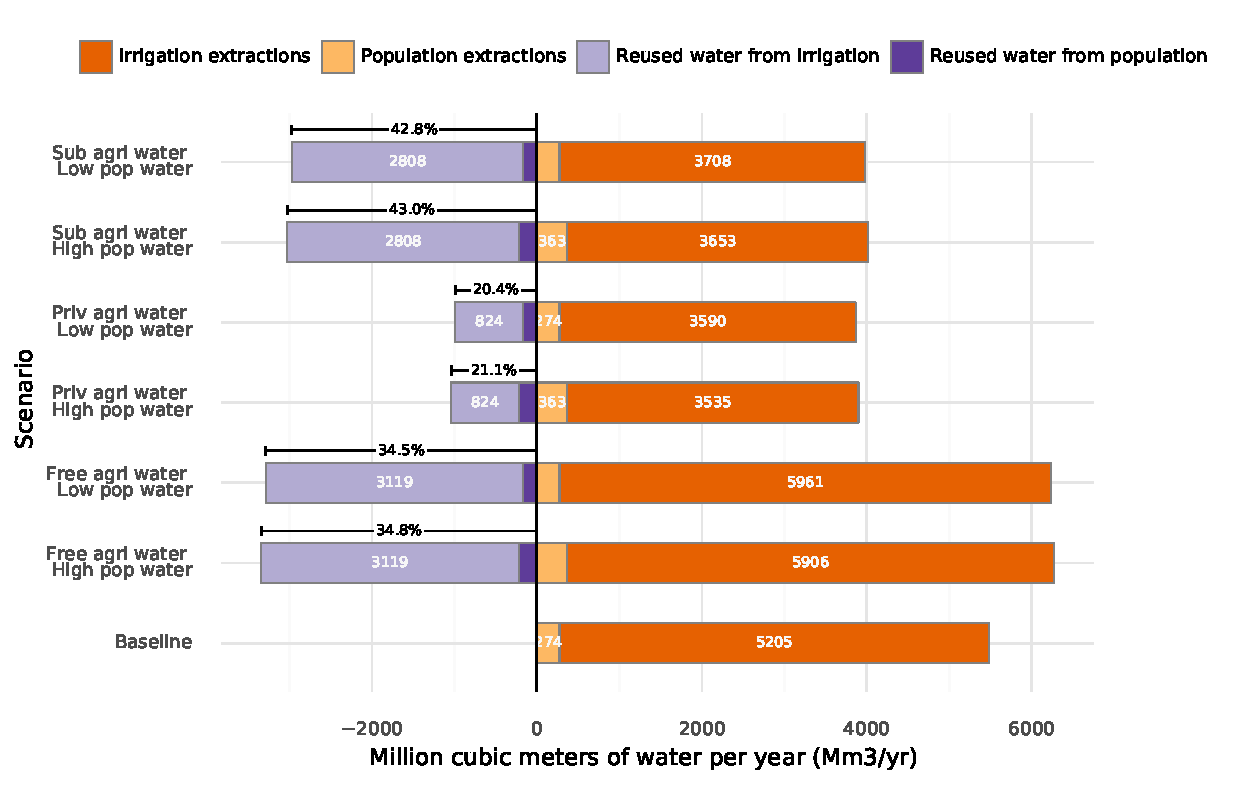
\includegraphics[width=0.8\textwidth]{Water}
	\caption{Water usage for all scenarios. At left: reused water after reclaim, treatment and allocation classified by population and irrigation source. Percentage bars indicate the share of reused water against the total demand. At right: overall water extractions classified by population and irrigation use. Percentage bars indicate the percentage of water saved compared to Baseline withdrawals}
	\label{fig:water}
\end{figure*}

On the other hand, the free agricultural water regime yielded much larger water extractions, even with water reuse. In fact, the share of reused water accounted for around 34\% of the water usage, lower share than that of the subsidized regime. This was due to the cap set to the on-farm storage area of maximum 2\% share of the cropland area. Therefore, while more recoverable water is available in the free water regime, the storage system cannot hold everything. This could be solved by setting a higher value for the permissible on-farm storage area, however, this would mean that more agricultural area would be used for storage purposes, possibly having trade-offs with target 2.3 of SDG 2 on doubling agricultural productivity and incomes of small-scale food producers.

Population water levels do not cause meaningful variations in the overall water use, as agricultural water needs are much more extensive. Nonetheless, with the use of more efficient irrigation schemes, the recoverable water from irrigation drainage decreases, thus populations treated wastewater share on agricultural water usage increases (synergies between SDG 6 and SDG 2).

\subsection{Least-cost wastewater treatment systems}
The least-cost treatment systems obtained for the low and high population water scenarios, share similarities in the combination of technologies identified and. Extended aeration, rotating biological contractors and intermittent sand filter were the least-costly technologies chosen. Nonetheless, differences in the technology shares exist. In the low population water requirements scenarios, wastewater was treated by intermittent sand filters, rotating biological contractors and extended aeration by 4\%, 21\% and 75\% share respectively. Whereas, in the high population water requirements scenario this shares were 2\%, 11\% and 87\%. In general, when lower capacity is required simpler treatment technologies are more cost-effective, as the independent variable of the CAPEX and OPEX cost functions is the available reclaimed wastewater flow.

% \begin{figure*}[!ht]
% 	\centering
% 	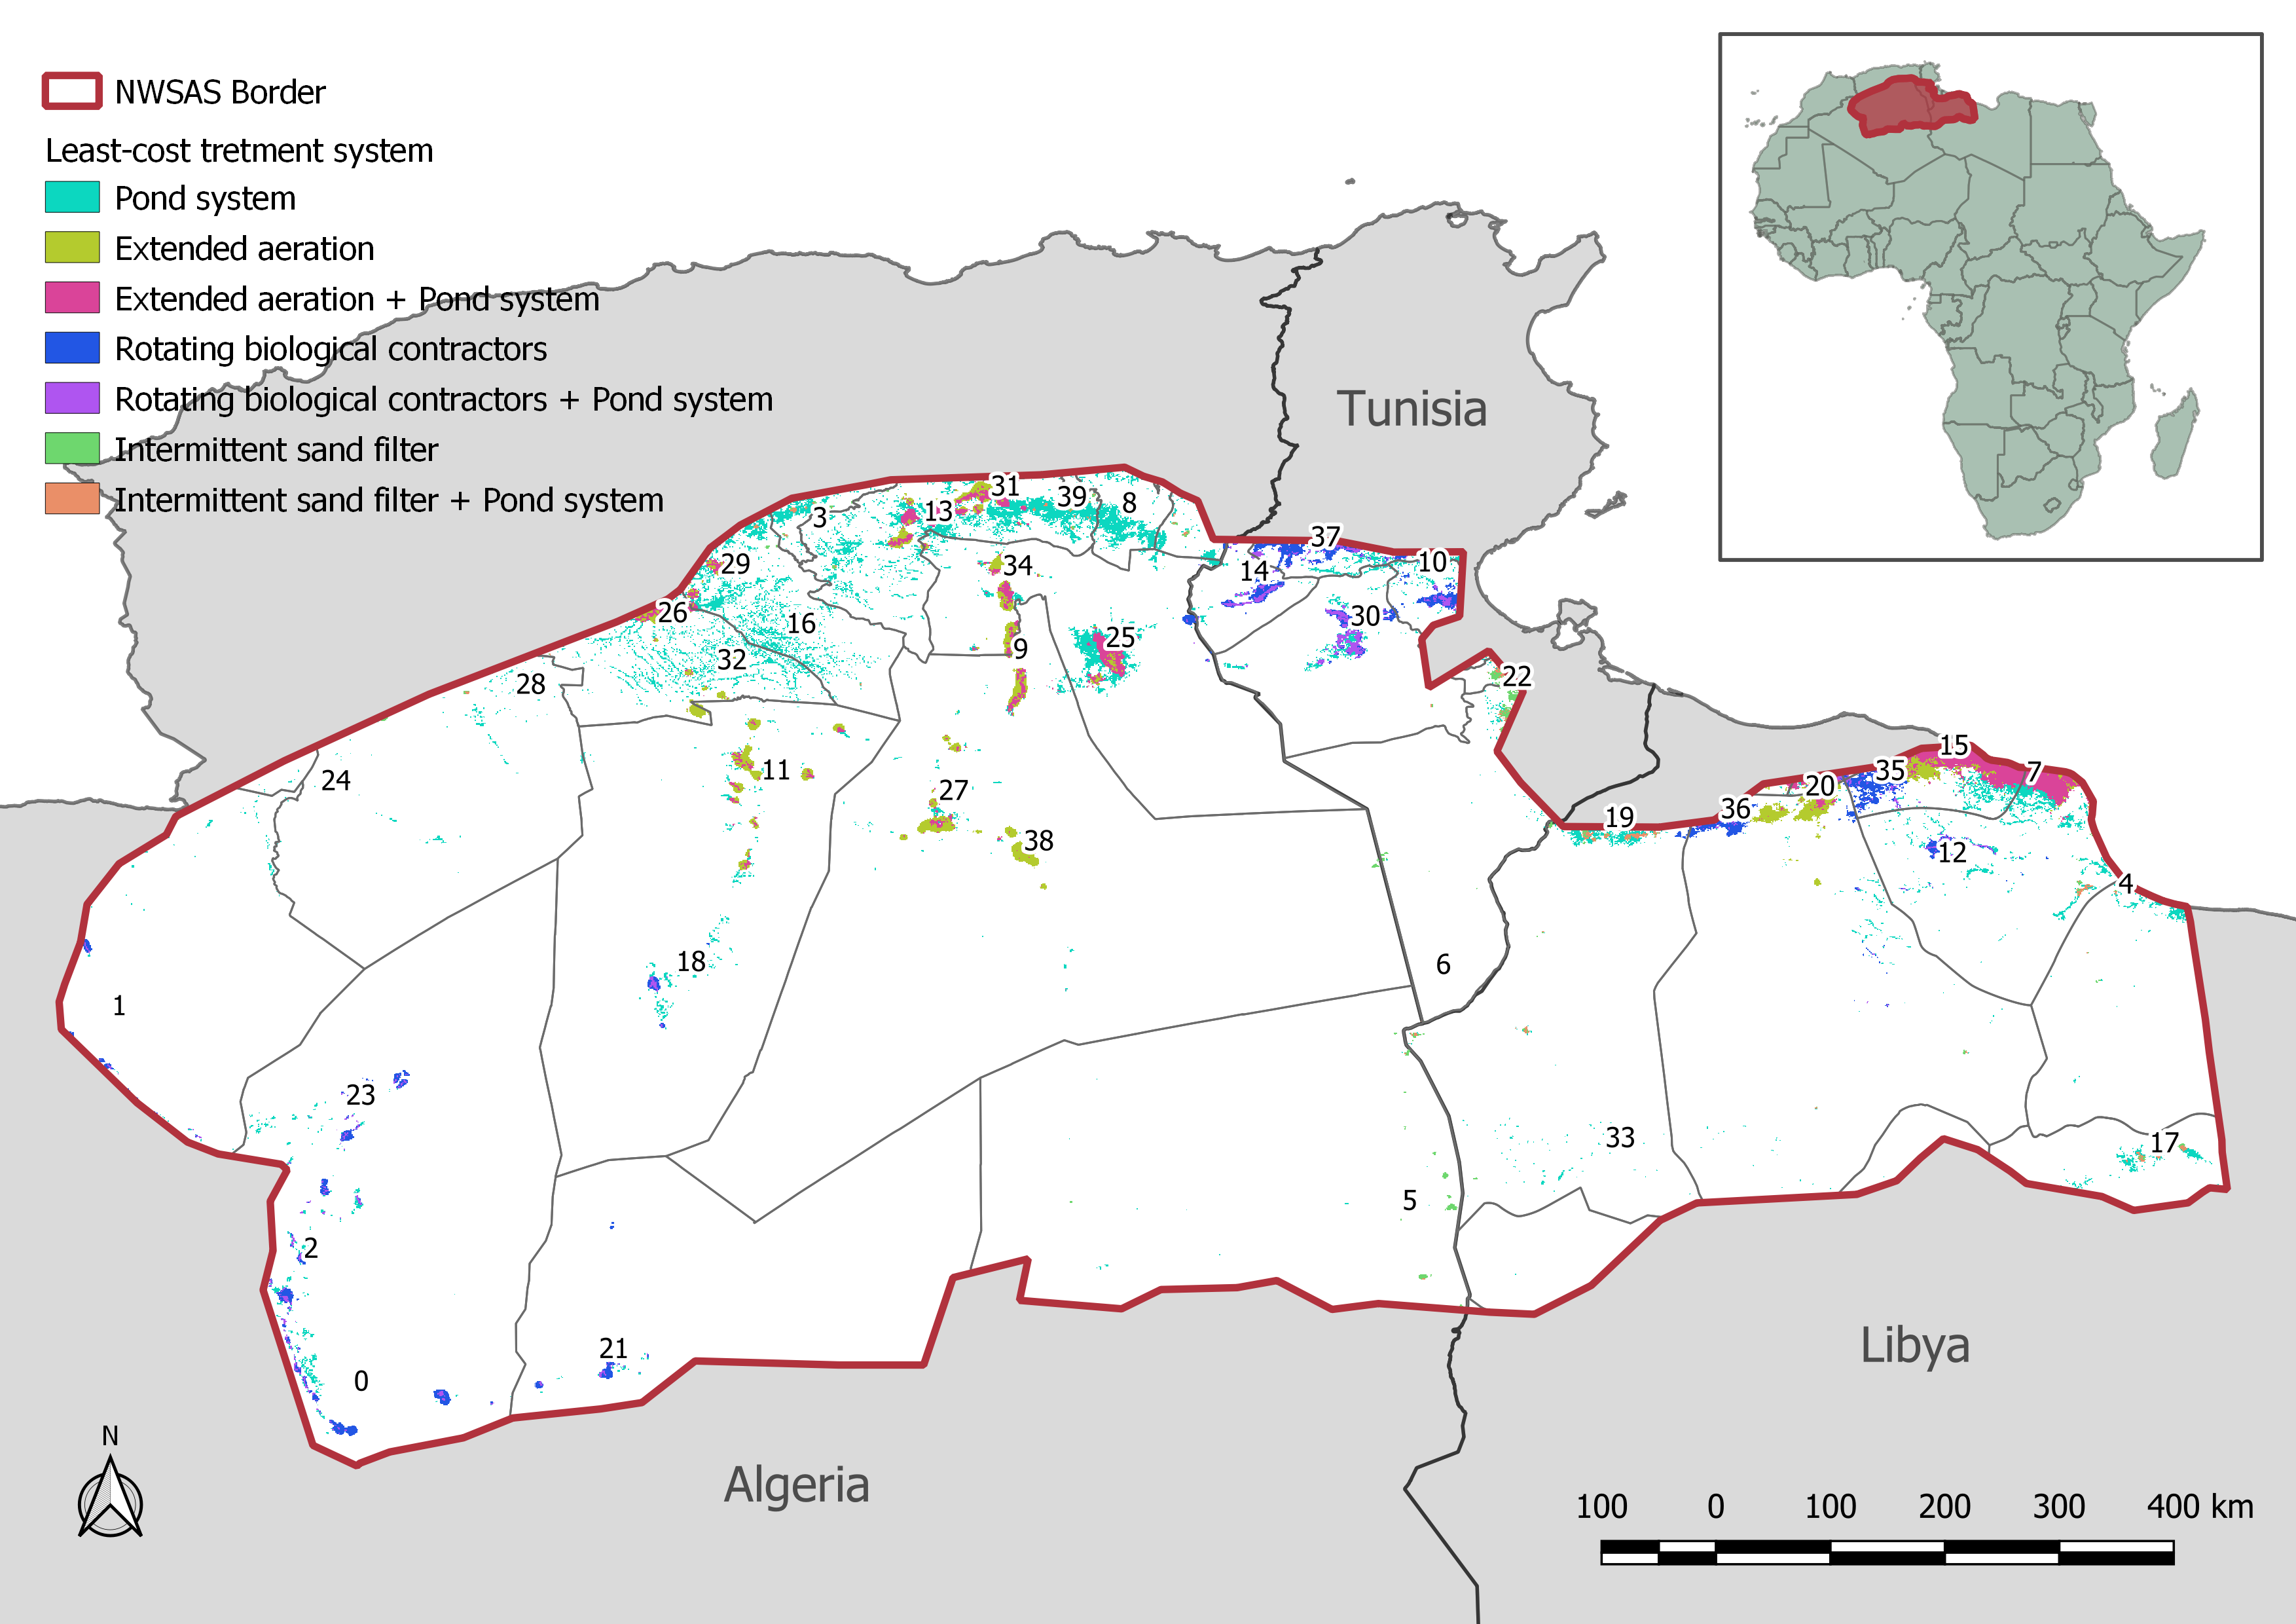
\includegraphics[width=0.88\textwidth, cfbox=black 1pt 0pt]{NWSAS_least-cost_system_cluster}
% 	\caption{Least-cost wastewater treatment options per cluster---low population water requirements.}
% 	\label{fig:leastLow}
% \end{figure*}

% \begin{figure*}[!ht]
% 	\centering
% 	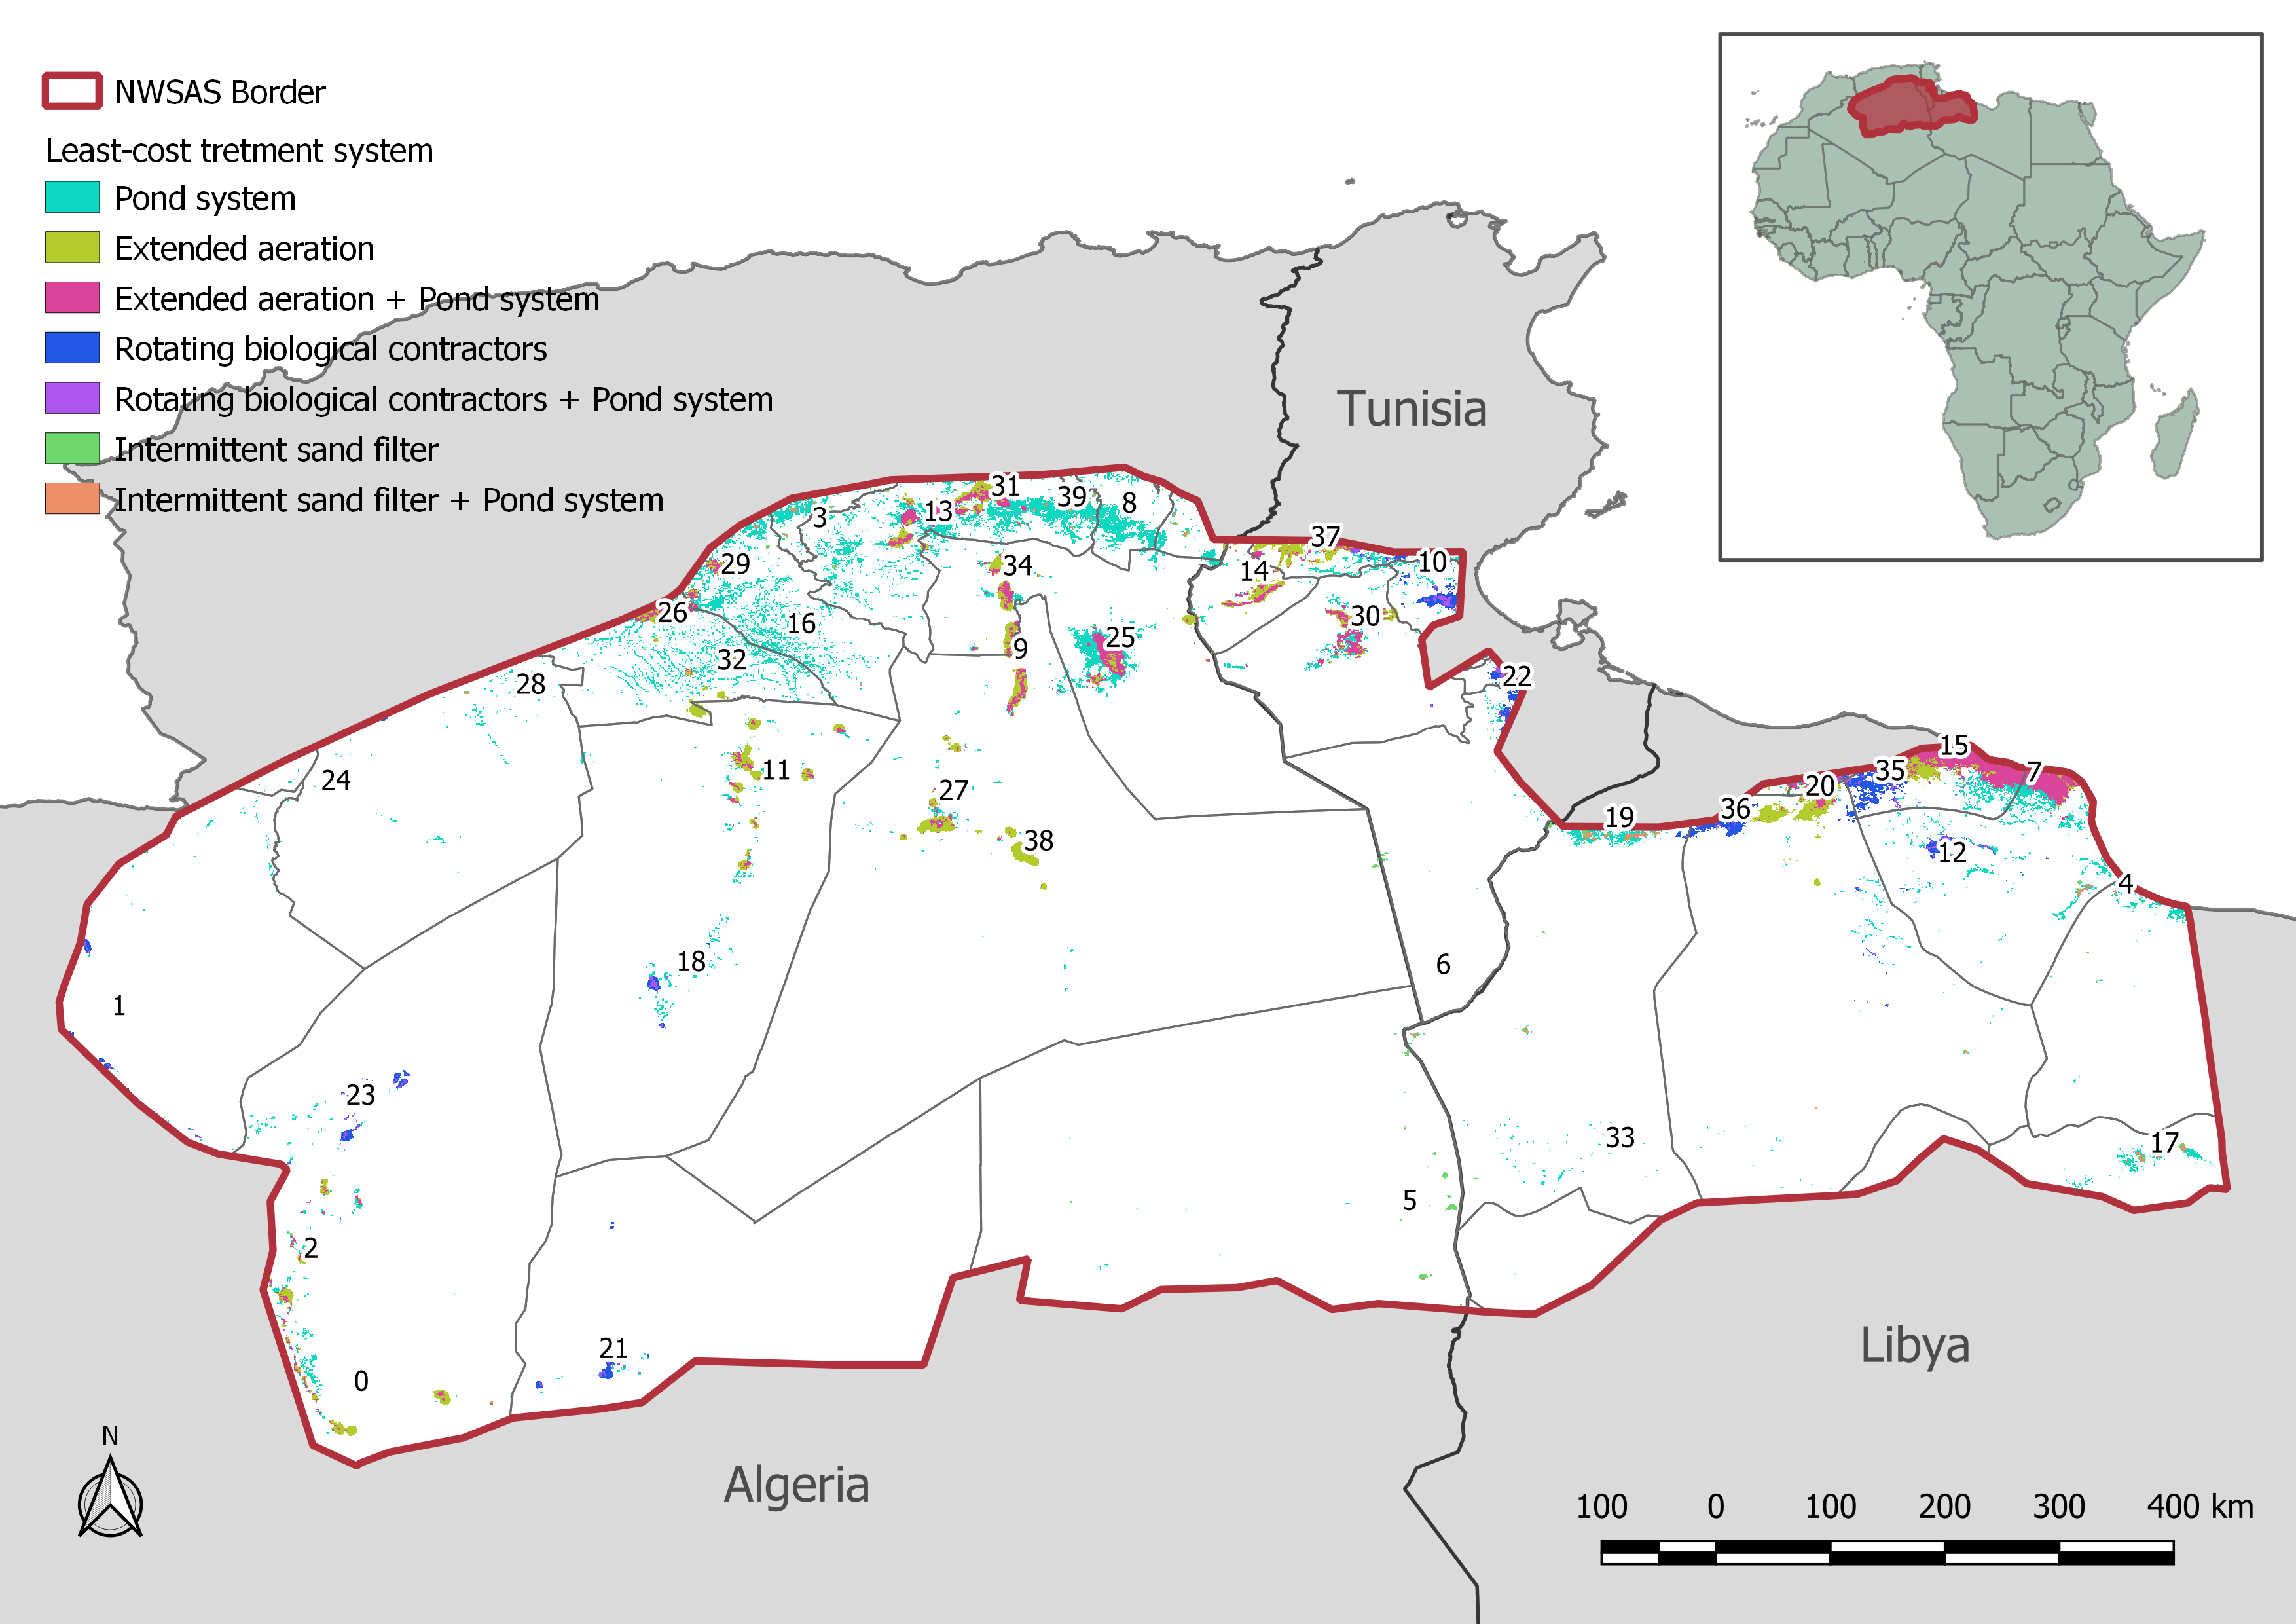
\includegraphics[width=0.88\textwidth, cfbox=black 1pt 0pt]{NWSAS_least-cost_system_cluster_high}
% 	\caption{Least-cost wastewater treatment options per cluster---high population water requirements.}
% 	\label{fig:leastHigh}
% \end{figure*}

The previous is important, as the amount of wastewater available from the agglomerations is key for the calculation of the least costly technology. Therefore, with larger agglomerations, scalable and higher capacity systems could be implemented. The downside however, is that if the costs related to the conveyance system are not evaluated, then the distances among population and/or irrigation points become irrelevant, which is arguably far from reality. Thus, the analysis of more compact clusters, reduces the drawbacks of not calculating the costs related to a wastewater conveyance system.

\begin{figure*}[!t]
	\centering
	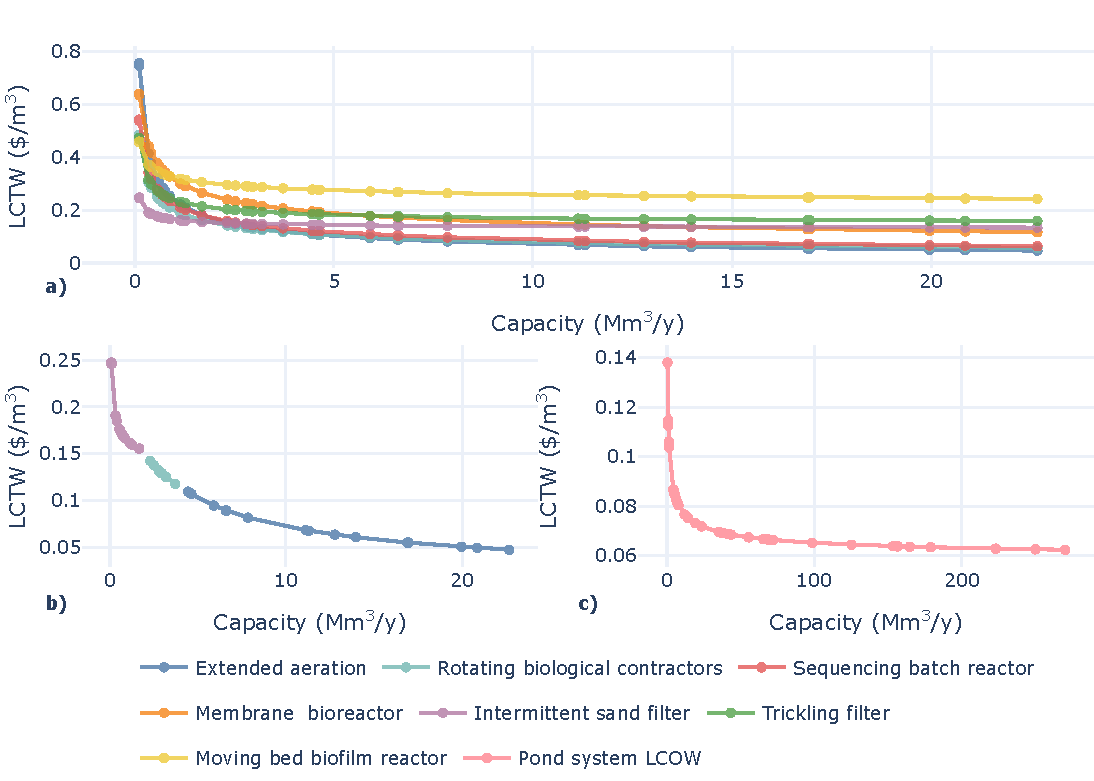
\includegraphics[width=0.9\textwidth]{lcowPopAg}
	\caption{Levelized cost of treated water (LCTW) against treatment capacity in the Baseline scenario. \textbf{a)} LCTW for the 7 different technologies evaluated for population wastewater treatment. \textbf{b)} Least-cost technologies for population wastewater treatment. \textbf{c)} LCTW of the pond systems treatment technology evaluated for agricultural tailwater.}
	\label{fig:lcowbaseline}
\end{figure*}

Overall, the least-cost treatment systems obtained, show an important trade-off, as the best solution is dependent from geospatial factors than can render a specific technology less costly than other in a given region. For example, clusters 0, 2, 37, 30 and 14 use rotating biological contractors in the low population water requirements scenarios, whereas extended aeration in the high population water scenario. Similarly, cluster 22 passes from using intermittent sand filters to biological rotating contractors in the same scenarios.

\subsection{Energy requirements}
Yearly energy requirements for agricultural irrigation are shown in \fref{fig:energyclusters} and additional results can be found in section 11 of the \textit{supplementary information}. The energy demand is considerably larger for the three countries in the northern part of the aquifer (i.e. clusters 7,  8, 25, 30, 31, 14, 13 and 39). This is mainly due to the intense agricultural activity of those regions. However, as shown in \fref{fig:energyclusters}, energy requirements are also affected by depth to groundwater and desalination needs due to TDS contents of the water. The depth to groundwater has a stronger impact on the overall energy requirements, as can be evidenced by clusters 29, 26, 3, 15, 13 and 7, all having lower depth values and being consistently placed to the right side of the diagonal. The opposite is true for clusters 9, 16, 39, 14, 31, 30, 25 and 8, all having higher depth levels, thus, higher energy requirements per cubic meter of water extracted. On the other hand, TDS content seems to have a much weaker effect. This suggests that, increasing water table levels is a important parameter to take into account for energy supply planning. It can significantly affect pumping energy requirements, but as well reduce the water productivity of the region. Nonetheless, reduced quality levels of water (i.e. higher TDS content) could have severe consequences on health and crop productivity, variables that were not accounted for in this study.

\begin{figure*}[!t]
	\centering
	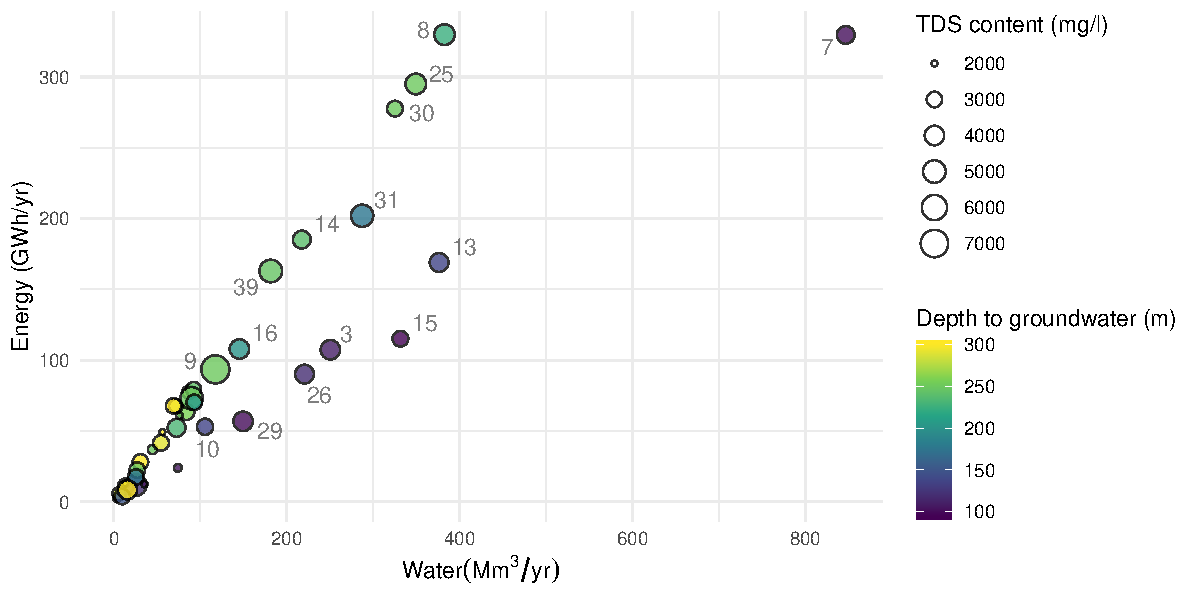
\includegraphics[width=\textwidth]{NexusPlot}
	\caption{Total energy and water requirements per cluster in the Baseline scenario. Clusters are represented by the data points and labeled by its number. TDS contents of water (mg/l) are shown as the size parameter of each data point/cluster. Depth to groundwater (m) is represented by the color ramp. The diagonal represents the trend line of the data points.}
	\label{fig:energyclusters}
\end{figure*}

The overall energy related outcomes for all scenarios are shown in \fref{fig:energy}. The energy requirements for groundwater pumping represent the major part of all three activities. Desalination energy, although considerable, is much smaller than pumping energy, this mainly due to the medium TDS levels found throughout the groundwater aquifer---in the 500 - 5000 mg/l in most of the area, see section 7 of the \textit{supplementary information} for more detail. All scenarios apart from the free agricultural water ones, reduced overall energy consumption compared to the Baseline. Such reductions, are achieved by the reuse of treated wastewater in irrigation, as the energy intensity of treatment is substantially lower than the energy intensity for pumping water from the deep aquifer. This shows synergies between SDG 6, SDG 2 and SDG 7, as when more wastewater is collected and treated it can be made available for reuse in agriculture, supporting sustainable food production and efficient irrigation schemes. Moreover, it can reduce energy intensity of the system and promote the use of clean energy sources.

\begin{figure*}[!t]
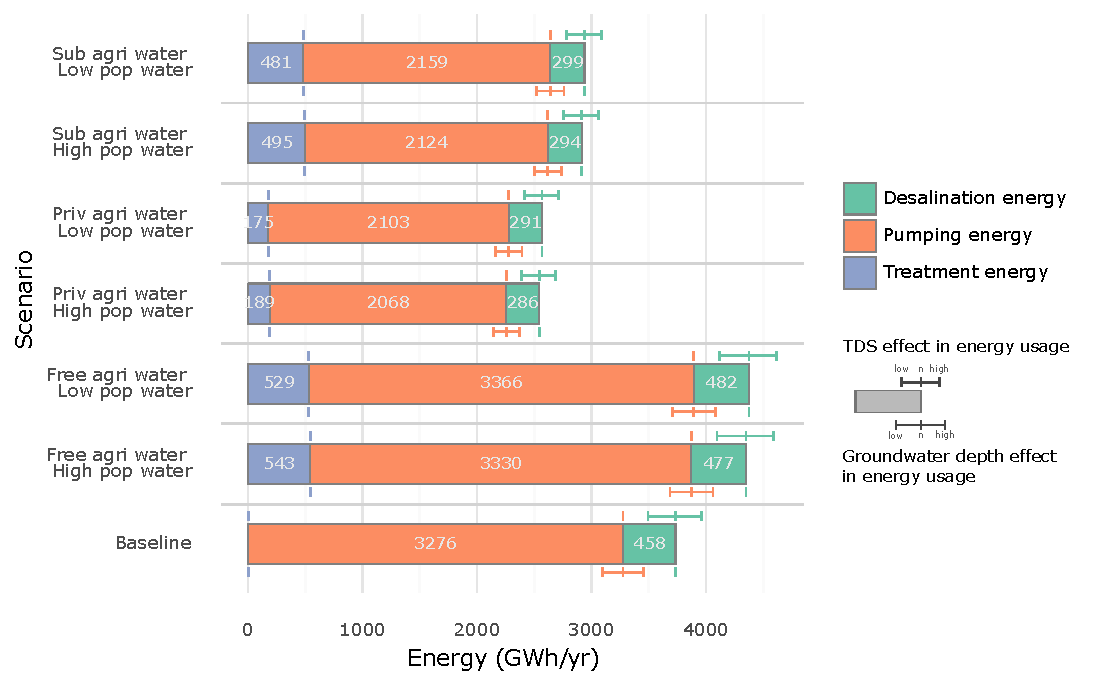
\includegraphics[width=\textwidth]{Energy}
\caption{Energy requirements for all scenarios with TDS and groundwater depth sensitivity analysis. TDS levels correspond to: $low=0.5\times n$ and $high=1.5\times n$; and groundwater depth levels correspond to: $low=n-10$ and $high=n+10$ meters.}
\label{fig:energy}
\end{figure*}

\subsection{Groundwater Stress}
The Groundwater Stress Indicator was computed aggregating the entire aquifer area (\fref{fig:gws}). A value of 5.01 in the Baseline scenario was obtained, which falls inside the medium-to-high stress category---however, it is known that the stress level in some parts of this area can reach to the extremely high category \cite{herbertGlobalAssessmentCurrent2019}. The private and subsidized agricultural water scenarios, presented a Groundwater Stress Indicator in the category of low-to-medium stress, which suggests a successful reduction on groundwater stress levels. However, the outcomes obtained for the free agricultural water scenarios, are higher at 5.68 and 5.65. Such increase in the stress, is due to the higher water requirements for agricultural irrigation. Synergies and trade-offs within SDG 2 with SDG 6 are clear, specially with targets 6.4 on increasing water-use efficiency and ensuring sustainable withdrawals and supply of freshwater to ease water scarcity and 6.6 on protect and restore water-related ecosystems.
\begin{figure}[!h]
	\centering
	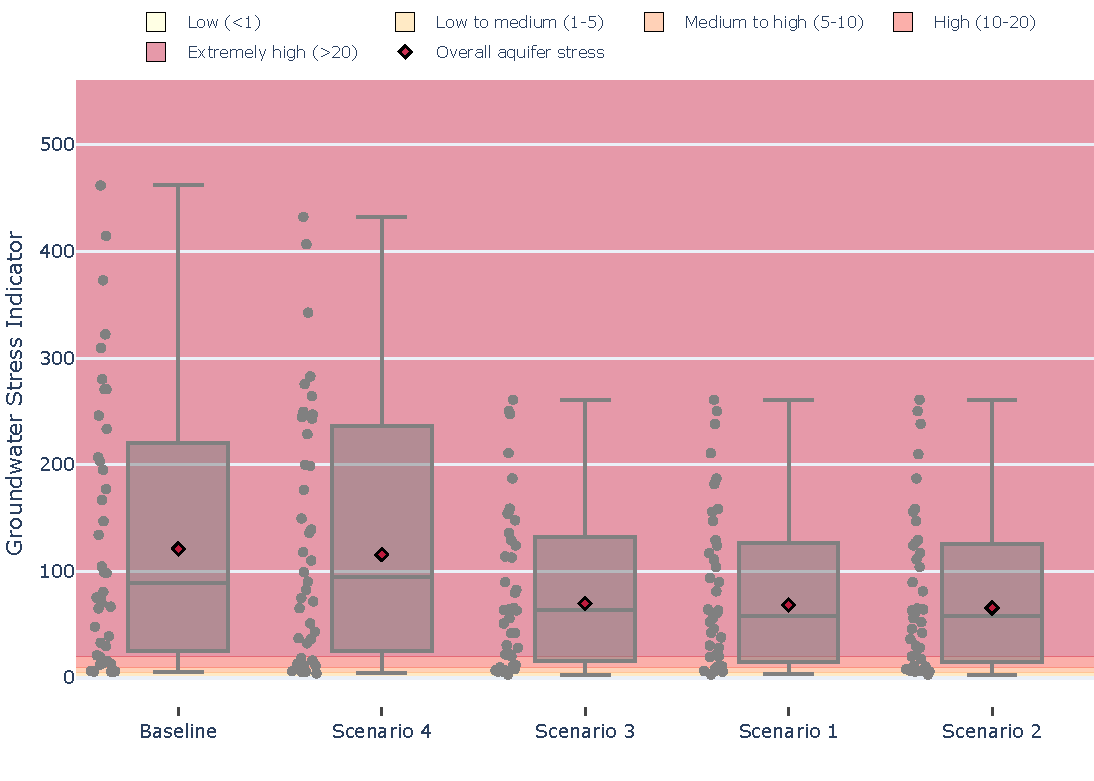
\includegraphics[width=0.9\textwidth]{GWS}
	\caption{Groundwater stress indicator for all scenarios.}
	\label{fig:gws}
\end{figure}

\begin{table}[!ht]
	\caption{\label{tbl:results}Summary of results by scenario. Selected results are calculated for the entire aquifer (total) and the minimum (min), maximum (max), average (mean) and median of the cluster results.}
	\footnotesize
	\lineup
\begin{tabular*}{\textwidth}{@{}*{7}{l}}
\br
                        &        & \centre{5}{Scenario} \\
 \ns
                        &        & \crule{5} \\
              Parameter & Value  &  Baseline &  Scenario 1 &  Scenario 2 &  Scenario 3 &  Scenario 4 \\
\mr
Water withdrawals (MCM) & total  &    6185.7 &      3404.9 &      3302.5 &      3589.5 &     \m6085.4 \\
                        & min    & \0\0\01.1 &   \0\0\01.1 &   \0\0\01.1 &   \0\0\01.1 &  \0\0\0\m1.1 \\
                        & max    &   \0617.1 &     \0351.8 &     \0351.8 &     \0355.9 &    \0\m631.4 \\
                        & mean   &   \0154.6 &    \0\085.1 &    \0\082.6 &    \0\089.7 &    \0\m152.1 \\
                        & median &   \0106.2 &    \0\066.0 &    \0\066.0 &    \0\070.9 &    \0\m103.5 \\
     Water reused (MCM) & total  &    2679.9 &      2679.9 &      1702.8 &      3558.1 &     \m3675.5 \\
                        & min    & \0\0\00.0 &   \0\0\00.0 &   \0\0\00.0 &   \0\0\00.0 &  \0\0\0\m0.0 \\
                        & max    &   \0289.0 &     \0289.0 &     \0200.3 &     \0393.1 &    \0\m393.1 \\
                        & mean   &  \0\067.0 &    \0\067.0 &    \0\042.6 &    \0\089.0 &   \0\0\m91.9 \\
                        & median &  \0\039.9 &    \0\039.9 &    \0\019.5 &    \0\049.1 &   \0\0\m62.2 \\
    Water savings (MCM) & total  & \0\0\00.0 &      2780.7 &      2883.2 &      2596.1 &    \0\m100.3 \\
                        & min    & \0\0\00.0 &   \0\0\00.0 &   \0\0\00.0 &   \0\0\00.0 &  \0\0\0-29.3 \\
                        & max    & \0\0\00.0 &     \0289.0 &     \0289.1 &     \0264.4 &   \0\0\m66.0 \\
                        & mean   & \0\0\00.0 &    \0\069.5 &    \0\072.1 &    \0\064.9 &  \0\0\0\m2.5 \\
                        & median & \0\0\00.0 &    \0\042.0 &    \0\042.0 &    \0\039.9 &  \0\0\0\m2.8 \\
           Energy (GWh) & total  &    4775.5 &      3048.5 &      2851.3 &      3235.0 &     \m5141.3 \\
                        & min    & \0\0\01.0 &   \0\0\01.1 &   \0\0\01.1 &   \0\0\01.1 &  \0\0\0\m1.1 \\
                        & max    &   \0553.5 &     \0359.2 &     \0341.3 &     \0376.1 &    \0\m608.7 \\
                        & mean   &   \0119.4 &    \0\076.2 &    \0\071.3 &    \0\080.9 &    \0\m128.5 \\
                        & median &  \0\075.8 &    \0\055.0 &    \0\054.5 &    \0\058.1 &   \0\0\m89.0 \\
 Groundwater stress (-) & total  &    6525.4 &      3823.2 &      3728.8 &      3961.6 &     \m6491.9 \\
                        & min    &  \0\0\03.4 &  \0\0\02.5 &   \0\0\02.5 &   \0\0\02.5 &  \0\0\0\m2.5 \\
                        & max    &   \0486.2 &     \0249.0 &     \0249.0 &     \0270.1 &    \0\m481.7 \\
                        & mean   &   \0163.1 &    \0\095.6 &    \0\093.2 &    \0\099.0 &    \0\m162.3 \\
                        & median &   \0130.2 &    \0\068.6 &    \0\068.6 &    \0\074.7 &    \0\m125.5 \\
      Water stress (\%) & total  &   \0561.1 &     \0308.9 &     \0299.6 &     \0325.6 &    \0\m552.0 \\
                        & min    &  \0\010.7 &   \0\0\07.9 &   \0\0\07.9 &   \0\0\07.9 &  \0\0\0\m7.9 \\
                        & max    &    1553.0 &     \0795.3 &     \0795.3 &     \0862.7 &     \m1538.8 \\
                        & mean   &   \0521.1 &     \0305.3 &     \0297.8 &     \0316.4 &    \0\m518.4 \\
                        & median &   \0416.0 &     \0219.1 &     \0219.1 &     \0238.5 &    \0\m400.8 \\
\br
\end{tabular*}
\end{table}

\subsection{Sensitivity analysis}
The sensitivity analysis demonstrates how a change of \rpm10 meters in the depth to groundwater level, has an average variation of circa \rpm5.5\% over the overall pumping energy requirements. Moreover, desalination energy requirements showed variations of $-$53\% to $+$50\%, when changes of \rpm50\% in the TDS levels were considered.

These effects on the energy-for-water requirements, are necessary to be assessed when planning for new water policies and water management strategies. Accordingly, accounting for new energy infrastructure, or potential energy savings could be key for the success of a new policy or solution to the water scarcity problem.